\begin{summary}
\section{Contexte}
Ce laboratoire a servi d'introduction à la programmation temps réel sur
système embarqué (ici STM32).
Le but était d'implémenter un Execution Framework (XF), en architecture IDF (sans
couche RTOS) pour simplifier le développement.
Notre XF se doit d'être portable, avec une implémentation sur PC avec
la librairie Qt, et une autre sur système embarqué STM32. Des tests communs aux deux
systèmes sont fournis, ainsi qu'une structure de base du projet.
\end{summary}

\section{XF}
Le XF (execution framework) est un framework servant à piloter plusieurs machines
d'états finies en pseudo-parallèle. Pour cela, il utilise des événements qui sont générés
par les machines d'états, qui passent par un Dispatcher avant d'être redistribué.
\begin{figure}[H]
    \centering
    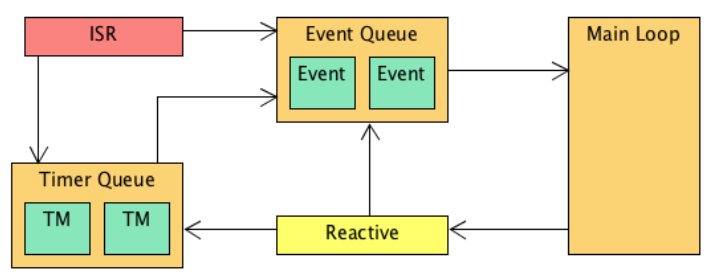
\includegraphics[width=0.75\textwidth]{Images/xf/IDF.PNG}
    \caption[Schéma de principe de notre XF en IDF]{Schéma de principe de notre XF en IDF (provenant du \emph{Cours XF}\footnotemark)}
\end{figure}
\footnotetext{\cite{coursXF}}
Dans notre cas, le XF fonctionnera directement sur le hardware, et tournera grâce
aux interruptions systèmes (architecture IDF). Ce cas est opposé d'un XF tournant
par-dessus un Real Time OS (architecture OXF). L'implémentation est plus simple, mais 
l'efficacité à grande échelle est réduit.

\begin{figure}[H]
    \centering
    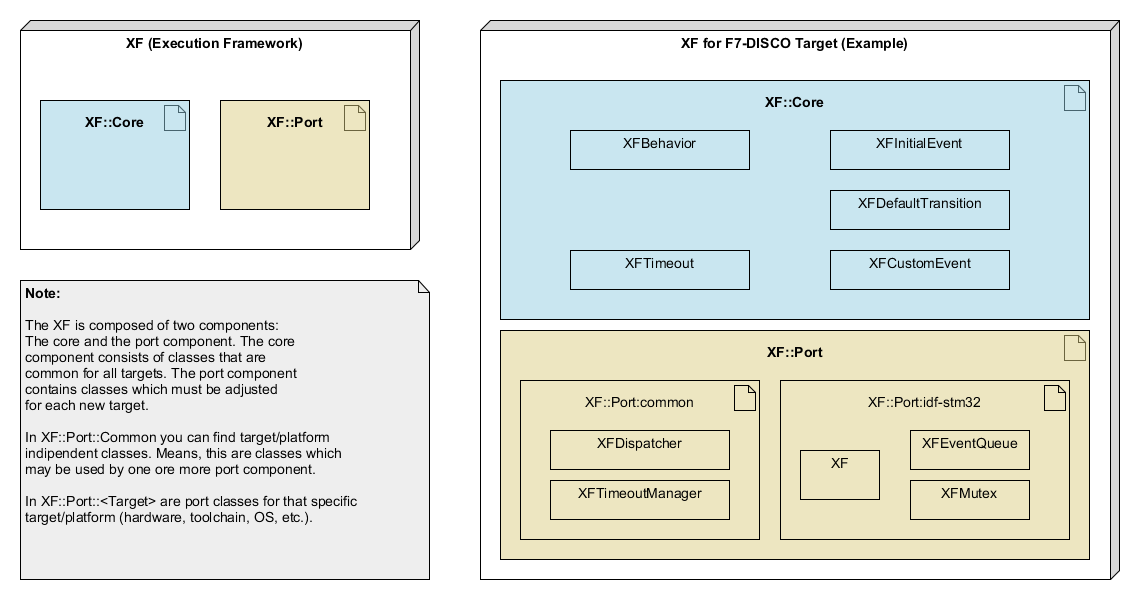
\includegraphics[width=\textwidth]{Images/xf/comp-simple-xf.png}
    \caption[Diagramme de composant de classe du XF]{Diagramme de composant de classe du XF 
        (provenant de la documentation \emph{Simplified XF}\footnotemark)}
\end{figure}
\footnotetext{\cite{documentation}}
Notre implémentation du XF se veut portable. Il a donc était séparé en deux parties :
\begin{itemize}
    \item XF::Core -> Contient le cœur du XF (machines d'état, événements), 
            cette partie restera inchangée sur tous les systèmes.
    \item XF::Port -> Contient les différents ports du XF, certains de ses ports
            seront spécifiques à chaque système (ex: XFMutex qui bloque les interruptions 
            sur système embarqué, et qui est un Mutex classique sur PC)
\end{itemize}
Le cœur et les ports forment ensemble un XF complet.
La majeur partie du XF::Core est déjà implémentée. Les événements restent à préciser.